\chapter{PROTOCOLOS DE COMUNICAÇÃO}

A comunicação envolve a troca de uma série de mensagens entre duas entidades. Parte
fundamental para a comunicação bem sucedida é a premissa a respeito das informações
transmitidas e recebidas, como por exemplo a linguagem e o meio de transmissão. Caso
as entidades envolvidas na comunicação não concordem em relação a estas premissas,
não será possível estabelecer um diálogo adequada.

Restrições a respeito do formato, meios de transmissão, e ações a serem tomadas no
envio e recebimento de mensagens são definidas por meio de protocolos. A partir do
momento em que duas entidades sigam o mesmo protocolo, pode-se garantir que a
comunicação será estabelecida. Assim como qualquer outra entidade, componentes de
\textit{hardware} e \textit{software} também estão sujeitos a protocolos de
comunicação \cite{kurose2012}.

Também é importante indicar que protocolos definem apenas as regras envolvidas em
uma troca de mensagens. Desde que as entidades cumpram as restrições, portanto
adotando a interface proposta, a estratégia de implementação se torna arbitrária.



\section{SUÍTES DE PROTOCOLOS}

No contexto da computação, redes de comunicação são construídas com diferentes
tecnologias de acordo com necessidades e restrições específicas, o que prejudica a
capacidade de intercomunicação entre dispositivos \cite{comer2000}. A Internet, por
exemplo, é uma coleção de redes menores que eventualmente utilizam tecnologias
diferentes, como é o caso de linhas telefônicas, e transmissão a rádio
\cite{tanenbaum2010}. Um desafio diferente é alcançar a intercomunicação em um
sistema complexo como tal, onde as redes que o compõem utilizam seus próprios
protocolos, desta vez específicos ao meio de transmissão.

De acordo com \cite{comer2000}, existem duas observações fundamentais ao projeto de
redes de comunicação:

\begin{enumerate}
  \item{Não existe nenhuma tecnologia de rede capaz de satisfazer às restrições de
        todos os possíveis contextos;}
  \item{Usuários desejam intercomunicação universal.}
\end{enumerate}

A primeira observação sugere que a necessidade de interoperabilidade eventualmente
surge pode surgir entre sistemas incompatíveis. Ainda assim, a discrepância deve ser
invisível ao usuário, que de qualquer forma espera a interoperabilidade, ponto
reafirmado pela segunda observação.

Esse tipo de interoperabilidade pode ser implementada tanto no nível das aplicações
quanto no nível da rede. Enquanto a primeira estratégia supõe que as aplicações
prevejam explicitamente suporte a cada uma das tecnologias, a segunda estratégia
é mapeada desde o \textit{hardware}, providenciando uma camada de abstração para os
componentes utilitários.

A intercomunicação no nível de rede (ou simplesmente internet \cite{comer2000})
também pode empregar um modelo de camadas. Neste caso, os protocolos são organizados
em uma hierarquia vertical, de acordo com seus objetivos. A interface entre cada
camada é bem definida, o que concede modularidade ao sistema \cite{kurose2012}.

Neste tipo de hierarquia as mensagens são enviadas sucessivamente da camada mais
superior até a camada mais inferior durante a transmissão, o inverso do que acontece
no recebimento. Apenas as camadas mais inferiores do transmissor e destinatário são
conectadas por meio de um meio de transmissão arbitrário, o que garante abstração do
meio para as camadas superiores.

\begin{figure}[h]
	\centering
		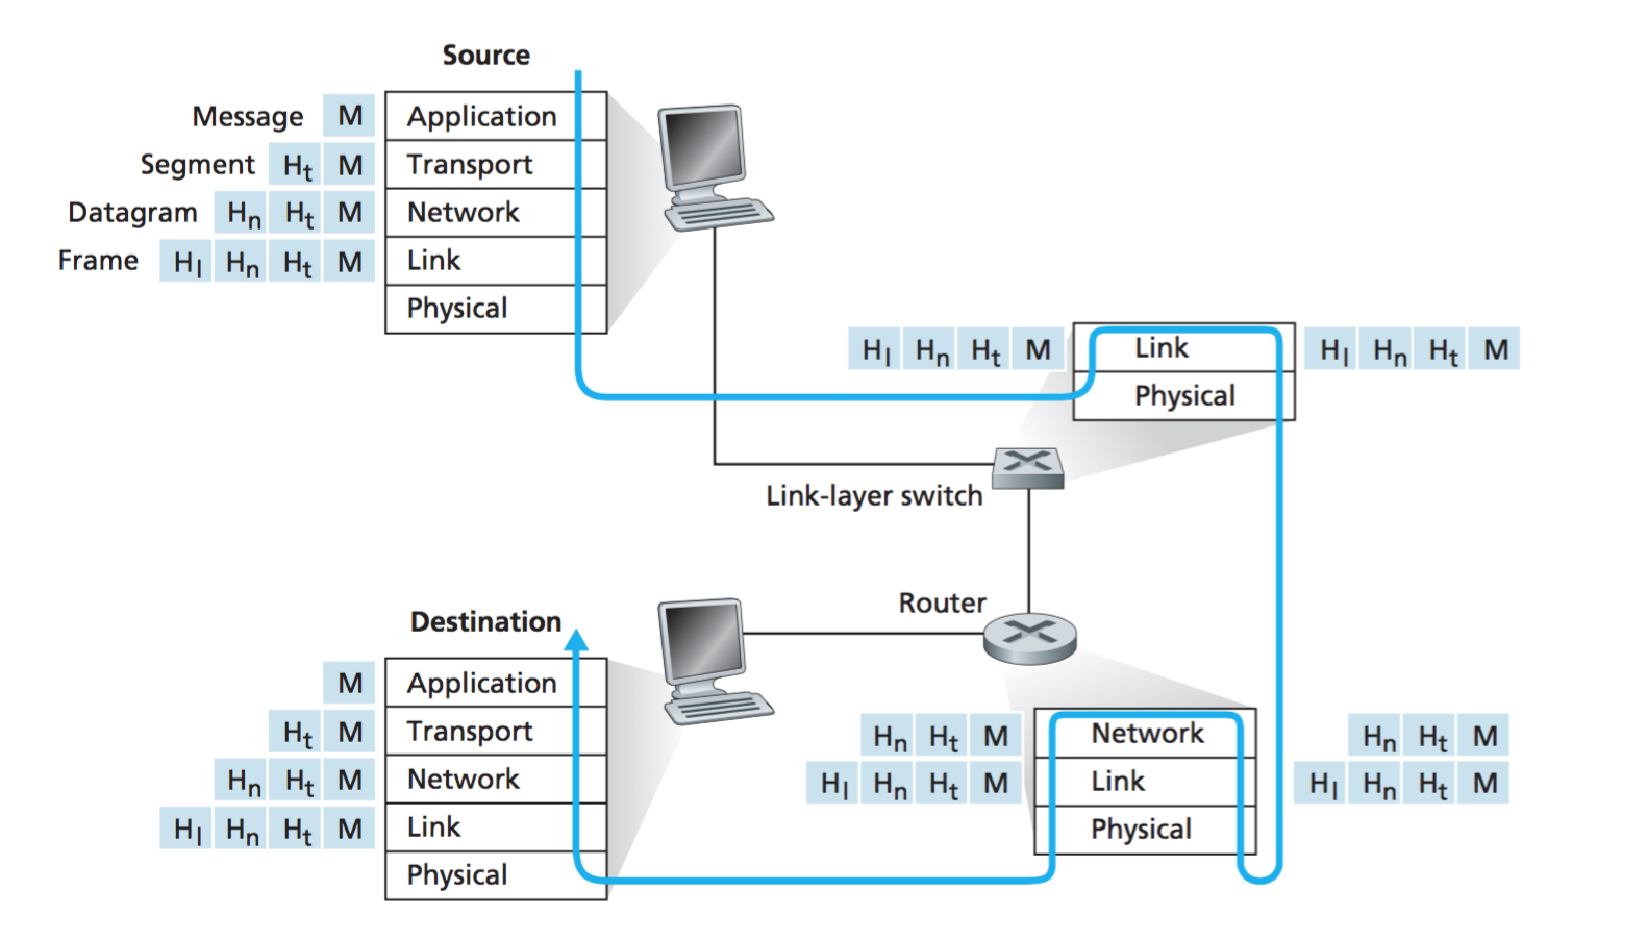
\includegraphics[keepaspectratio=true,scale=0.6]{figuras/encapsulamento.eps}
	\caption{Encapsulamento de mensagens em um modelo de camadas \cite{kurose2012}}
	\label{fig:encapsulamento}
\end{figure}

A figura \ref{fig:encapsulamento} mostra este processo no contexto do TCP/IP, também
conhecido como a suíte de protocolos da Internet. Neste caso, os protocolos de cada
camada adicionam um cabeçalho às mensagens recebidas do nível anterior, o que
permite a adição de informações adicionais destinadas ao mesmo protocolo
implementado no comunicante.

% TODO: exemplificar com o OStatus + referência
Apesar deste processo descrever a interação entre os protocolos organizados em um
modelo de camadas, uma estratégia semelhante é utilizada em outras suítes. Uma
família de protocolos da camada de aplicação, por exemplo, não segue nenhum dos
modelos de camadas de redes de comunicação, mas ainda assim utiliza os conceitos de
hierarquia e encapsulamento para garantir interoperabilidade e cumprir uma tarefa
específica em conjunto.



\section{PADRONIZAÇÃO DE PROTOCOLOS}

A definição de protocolos é apenas o primeiro passo para a intercomunicação de
sistemas. Se não existir um acordo a respeito da especificação utilizada será mais
difícil estabelecer a comunicação entre serviços \cite{kurose2012}. A padronização
garante o estabelecimento deste acordo.

O conceito de efeito de rede indica que a adoção de um protocolo se torna mais
valiosa à medida que um maior número de entidades também o utilize
\cite{liebowitz1998}. Justifica-se portanto o interesse em incentivar a padronização
de protocolos.

A partir do momento em que uma série de entidades entra em consenso a respeito da
especificação de um protocolo, estabelece-se um padrão \textit{de facto}. A
iniciativa de padronização também pode surgir através de entidades regulamentadoras,
como a Organização Internacional para a Padronização (ISO), ou a \textit{Internet
Engineering Task Force} (IETF), o que leva ao estabelecimento padrões \textit{de
jure} \cite{tanenbaum2010}.

O processo de definição de novos padrões \textit{de jure} depende da entidade
regulamentadora relacionada, e ocasionalmente parte de padrões \textit{de facto} já
utilizados na comunidade. Geralmente uma especificação é proposta, discutida, e
revisada pela entidade antes de se tornar um padrão, o que no caso da ISO pode levar
de seis meses a alguns anos \cite{tanenbaum2010}.

Propostas e padrões estabelecidos devem ser documentados de alguma forma. A IETF
adota o formato de \textit{Request for Comments} (RFC), publicações que descrevem
completamente uma especificação, e estão disponíveis a consulta pela comunidade.

Uma proposta deve cumprir uma série de requisitos antes de ser endossado por uma
organização. No caso da IETF, cada proposta passa por vários níveis de maturidade
até alcançar a categoria de padrão. Cada um destes níveis pode ser alcançado ao
satisfazer as recomendações de determinados grupo da comunidade. Um exemplo destes
requisitos é a exigência de uma prova de conceito de interoperabilidade, como uma
implementação de referência entre duas ou mais entidades distintas \cite{rfc1280}.


\subsection{Simple Mail Transfer Protocol}

A troca de mensagens na internet é um problema recorrente, envolve as questões de
interoperabilidade entre redes, e adoção de padrões para a comunicação entre
serviços. O esforço de padronização acontece desde a década de 70 com o \textit{Mail
Box Protocol}, e continua desde a definição do \textit{Simple Mail Transfer
Protocol}.

O SMTP é um protocolo para o transporte e entrega de mensagens de e-mail entre
processos. A especificação garante que a troca de mensagens aconteça entre clientes
que se localizam em redes diferentes, o que permite a construção de um serviço que
funcione de maneira confiável sobre a internet \cite{rfc2821}. Trata-se de um
protocolo amplamente adotado e formalmente padronizado desde 1982, portanto
interessante para ser analisado no contexto do estabelecimento de padrões.

Caracterizado como um protocolo orientado a conexões entre clientes e servidores, ou
transmissores e receptores, o SMTP é guiado por uma série de comandos predefinidos.
Os servidores também são responsáveis por retransmitir mensagens, caso não sejam os
destinatários finais \cite{kurose2012}.

A troca de mensagens geralmente acontece em um único salto após o estabelecimento de
uma conexão orientada entre o remetente e o destinatário. A retransmissão de
mensagens é uma alternativa, utilizada por exemplo em casos em que um usuário moveu
sua caixa de e-mails de um servidor para outro e deseja receber as mensagens no seu
novo endereço.

\begin{figure}[h]
	\centering
		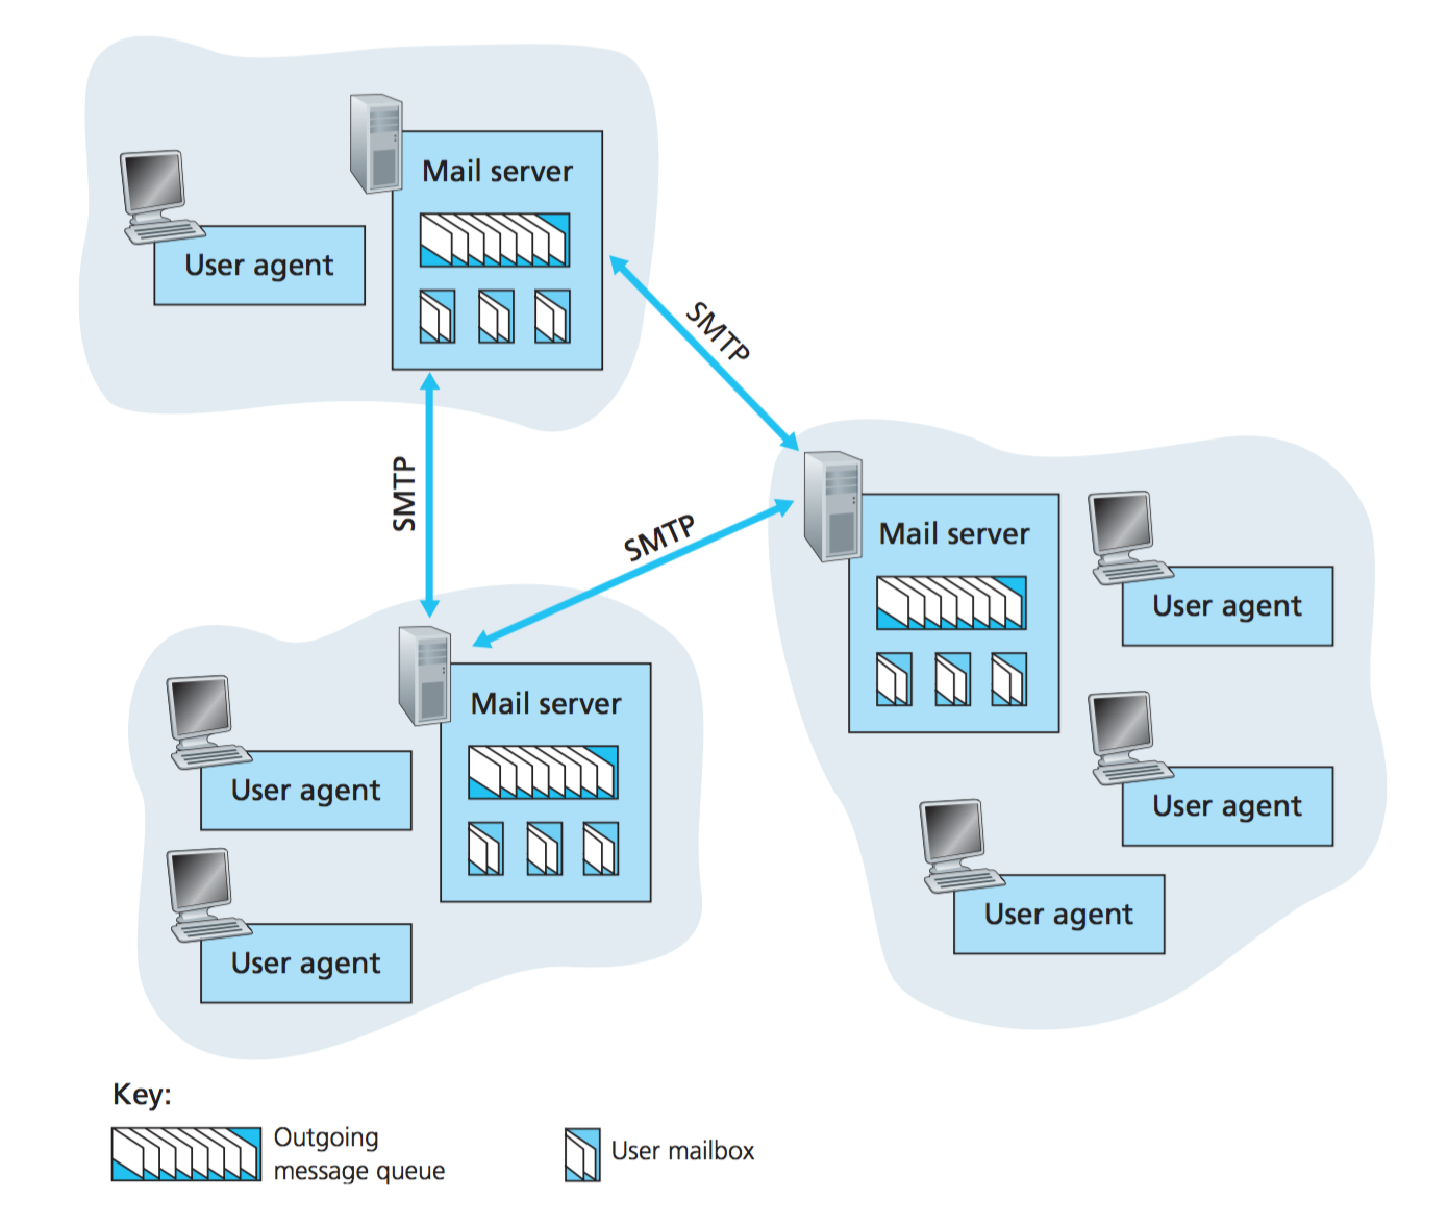
\includegraphics[keepaspectratio=true,scale=0.6]{figuras/smtp_internet.eps}
	\caption{Uma visão geral de um sistema de e-mails \cite{kurose2012}}
	\label{fig:smtpInternet}
\end{figure}

Como pode ser visto na figura \ref{fig:smtpInternet}, o SMTP é um protocolo
intermediário entre servidores de e-mail que alternam entre os papéis de transmissor
e receptor. Cada um destes servidores fornece a seus próprios clientes, constituindo
sistemas menores onde a interação não é necessariamente coberta pela especificação
do SMTP.

Cada um destes sistemas intermediários não é necessariamente compatível, visto que a
comunicação entre o servidor e o usuário depende das aplicações envolvidas, e
eventualmente utiliza outros padrões, como por exemplo POP3 ou IMAP no gerenciamento
de caixas de e-mail pessoais \cite{tanenbaum2010}.

Levando em cnsideração esta arquitetura descentralizada, pode-se indicar a
semelhança com o formato de sistemas federados. Qualquer novo sistema capaz de
implementar a especificação do SMTP torna-se parte da federação, onde a
heterogeneidade entre os sistemas intermediários é completamente transparente para
os usuários do serviço.

O SMTP foi definido em publicações da IETF, tendo sido proposto com base em
especificações anteriores. Trata-se de um padrão \textit{de jure} aberto, definido
por uma organização antes de ser adotado pelo mercado.



\section{PROTOCOLOS DE FEDERAÇÃO}

% TODO
% seção de fatores que dificultam a padronização da federação?

A inexistência de um protocolo padrão para a federação de mídias sociais dificulta
o desenvolvimento de aplicações interoperáveis. São enfrentados os mesmos problemas
identificados na intercomunicação de redes heterogêneas, já que os desenvolvedores
solucionam os problemas com tecnologias diferentes, de acordo com as próprias
restrições e necessidades.

Ainda que exista uma tendência da comunidade em adotar propostas de protocolos, o
que pôde ser observado no caso do projetos OStatus e Diaspora, abordagens
alternativas naturalmente serão desenvolvidas. A ausência de um protocolo bem
difundido segmenta a adoção por parte dos desenvolvedores, o que prejudica o efeito
de rede e impede o surgimento de um padrão \textit{de facto}.

Ao discutir a padronização da federação é interessante não só analisar o esforço da
comunidade em discutir e adotar propostas ainda não completamente estabelecidas,
como também identificar as questões que impediram o acordo. Antes disto, é
interessante apresentar os projetos que federação que ganharam maior visibilidade,
o OStatus e o Diaspora.


\subsection{OStatus}

O OStatus é um conjunto de protocolos que permite interação em tempo real entre
redes redes sociais. Foi inicialmente proposto por Evan Prodromou para a
implementação do StatusNet, que posteriormente deu origem ao projeto GNU Social.

Até certo ponto, tecnologias como o Atom e RSS permitem a interação entre sistemas,
mais especificamente no compartilhamento de conteúdo. No entanto, são restritas no
que diz respeito a interação em tempo real, problema que o OStatus propõe resolver
combinando \textit{feeds} Atom com uma série de outros mecanismos.

A especificação do OStatus propõe a utilização das tecnologias listadas a seguir.

\begin{itemize}
  \item{PubSubHubbub: mecanismo de inscrição e submissão}
  \item{WebFinger: descoberta de identidade}
  \item{Activity Streams: representação de atividades de usuários em redes sociais}
  \item{Salmon: descentralização de trocas de mensagens}
\end{itemize}

O projeto obteve visibilidade na comunidade, contando com uma das maiores
iniciativas de padronização. O OStatus chegou a se tornar alvo de um grupo de
trabalho da W3C em 2012, uma das maiores organizações de padronização para a
\textit{web}. Apesar disto, o grupo não apresentou avanços desde então, e o
desenvolvimento do projeto está estagnado.

\subsubsection{PubSubHubbub}

O PubHubSub especifica um sistema distribuído para publicação e assinatura de
conteúdos. A ideia é que serviços possam se inscrever em diretórios centrais (ou
\textit{hubs}), expressando o interesse em receber as atualizações em tempo real.
Este padrão complementa tecnologias como o RSS, que baseia a atualização apenas na
solicitação dos interessados.

Serviços inscritos devem identificar o tópico desejado através de URIs, e oferecer
um servidor disponível pela internet para que a notificação seja realizada. É de
responsabilidade de cada serviço notificar os \textit{hub} conhecidos a cada nova
publicação. Cada \textit{hub} é responsável por replicar a mensagem a todos os
serviços inscritos.

\subsubsection{WebFinger}

O WebFinger é um protocolo de descoberta de identidade que soluciona o problema do
compartilhamento de informações de usuários entre servidores remotos \cite{rfc7033}.
A proposta é que a partir de um atributo identificador e do endereço do servidor de
origem, seja possível garantir existência de um usuário e recuperar suas informações
públicas.

A especificação do WebFinger propõe que todos os recursos possam ser identificados
por uma URL, e que todas as solicitações e respostas sejam realizadas através de
requisições HTTP. Servidores que forneçam informações através do WebFinger devem
responder aos \textit{endpoints} definidos no protocolo com objetos JSON. Servidores
que pretendam consumir tais informações precisam conhecer apenas a URL do recurso de
interesse, o que pode ser encontrado a partir do identificador do usuário e do
domínio do servidor de origem (em um processo que pode ser classificado como LRDD
\cite{lrdd2010}). 

\subsubsection{Activity Streams}

O Activity Streams é uma especificação que propõe um formato para a representação
das atividades dos usuários em uma rede social. O objetivo é facilitar o consumo
destas ações para o resto da rede e serviços externos.

A especificação mais atual do Activity Streams propõe a representação em formato
JSON, definindo propriedades que identificam a ação, o usuário responsável, e a
entidade alvo. Especificações mais antigas utilizam o padrão Atom, com restrições
semelhantes em relação ao conteúdo das mensagens. O OStatus adota a especificação
baseada em Atom, utilizando mensagens em formato XML.

O padrão trata apenas da representação das mensagens, dependendo de outros
mecanismos para a distribuição das atividades. Geralmente são utilizadas APIs ou
\textit{feeds} em conjunto com mecanismos de inscrição.

\subsubsection{Salmon}

Combinar soluções como Atom e PubHubSub permite que conteúdos sejam publicados e
atualizados em tempo real. No entanto, a partir do ponto em que um conteúdo pode ser
consumido e atualizado a partir de um número arbitrário de serviços, também deve-se
investir esforço para garantir que o seu estado seja o mesmo em toda a rede.

O objetivo do Salmon é descentralizar a capacidade de contribuir com o estado de um
conteúdo, mas mantendo sua consistência por toda a federação. Para isto,
especifica a troca de mensagens entre o servidor de origem e todos os outros que
podem contribuir com o estado de um conteúdo, definindo o formato das mensagens, e
as diretrizes necessárias para agregar as atividades.

Um servidor que implemente o protocolo deve incluir a URL de um \textit{endpoint}
capaz de processar mensagens Salmon, enviadas para este endereço por qualquer
serviço interessado em modificar o estado de uma publicação. Uma mensagem Salmon se
trata de uma nova entrada no \textit{feed}, codificada em \textit{base64} e envolta
por outra estrutura envelope (geralmente XML) assinada digitalmente. Cabe ao
servidor processar as solicitações de acordo com suas próprias políticas.

\subsubsection{Estado do padrão}

O projeto OStatus deu um passo importante em direção à padronização com a criação do
grupo de trabalho na W3C. No entanto, a comunidade não conseguiu entrar em consenso
em relação às decisões do protocolo, principalmente no que diz respeito à
privacidade.

Não exitem avanços no projeto nos últimos anos, e o grupo de trabalho da W3C não
produziu nenhum relatório desde que foi criado. Em 2012 o fundador do projeto, Evan
Prodromou, anunciou o desenvolvimento do \textit{pump.io}, outro protocolo de
federação, abandonando o desenvolvimento do OStatus.

Ao mesmo tempo em que não existia comunidade ativa para a evolução do projeto, parte
das tecnologias utilizadas continuou a ser mantida, o que contribui para o seu
estado de obsolescência. O Activity Streams, por exemplo, já conta com uma segunda
especificação que suporte tecnologia JSON, enquanto o OStatus ainda considera a
especificação baseada em Atom.

% TODO: comentar sobre projetos novos que utilizam OStatus
% https://github.com/Gargron/mastodon


\subsection{Diaspora}

O projeto Diaspora surgiu com a intenção de implementar o conceito de redes sociais
descentralizadas em resposta aos problemas de liberdade e privacidade encontrados em
plataformas sociais privadas. Sua primeira versão foi lançada em Setembro de 2010
como fruto de uma campanha de financiamento coletivo, passando a ser completamente
governado pela comunidade a partir de Agosto de 2012.

A proposta dos desenvolvedores é evitar a centralização de conteúdo, portanto a
falta de controle sobre as informações, construindo uma rede de instâncias pessoais
da plataforma, ou \textit{pods}. Cada servidor Diaspora reúne apenas as informações
dos seus próprios usuários, mas em cooperação com outros \textit{pods} possibilita a
interação em uma rede federada.

O protocolo de federação do Diaspora foi definido para convergir com o OStatus assim
que o último passe a suportar o conceito de privacidade limitada, o que nunca
aconteceu. A implementação leva em consideração a troca de mensagens em formato XML,
respeitando alguns conceitos básicos como a existência de usuários remotos e
atualização remota e retransmissão.

\subsubsection{Usuários Remotos}

Um conceito fundamental para a implementação de redes federadas é considerar a
existência de usuários remotos. A maioria das aplicações só possui o conceito de
usuários locais, que estão diretamente autenticados no serviço e possuem todas as
informações na base de dados local. No entanto, ao possibilitar a interação com
usuários de outras redes, usuários externos ao sistema precisam ser explicitamente
considerados na implementação das funcionalidades.

O Diaspora conceitualiza seus usuários em locais e externos. Enquanto usuários locais
respeitam a definição tradicional, os usuários externos interagem com a aplicação
através dos mecanismos de federação. É importante prever a existência de usuários
externos na modelagem de sistemas. Por este motivo, implementar federação em
aplicações já consolidadas pode exigir um certo esforço de refatoração.

\subsubsection{Capacidade de Retransmissão}

A retransmissão é essencial em sistemas federados, visto que interações em uma rede
eventualmente devem afetar \textit{pods} relacionados. A restrição implementada pelo
Diaspora indica que todas as notificações neste contexto sejam entregues tanto aos
usuários locais quanto aos usuários remotos. Adicionalmente, a notificação de
usuários locais não deve depender da resposta dos demais \textit{pods}.

Em configurações de integração mais complexas, a capacidade de retransmissão passa a
ser um requisito essencial para a troca de mensagens. Considere uma situação
hipotética em que \textit{pods} \textbf{A} e \textbf{B} são federados com o
\textit{pod} \textbf{C}, mas não entre si. Qualquer modificação em um conteúdo de
\textbf{C} compartilhado com \textbf{A} e \textbf{B} deve afetar os três
\textit{pods}. No entanto, se a modificação partir de \textbf{A}, há uma dificuldade
em notificar \textbf{B}, visto que o \textit{pod} em questão só reconhece a
existência de \textbf{C}. A solução defendida pela implementação do Diaspora é que
\textbf{C} retransmita a notificação para todos os \textit{pods} com os quais o
conteúdo seja compartilhado. Isso garante que todos os sistemas federados envolvidos
em uma interação sejam notificados, contribuindo com consistência das informações.

\subsubsection{Troca de Mensagens}

O Diaspora define um conjunto de mensagens que delimitam as possíveis interações
entre \textit{pods}.

\begin{itemize}
  \item{Compartilhamento de informações}
  \item{Publicações de conteúdo}
  \item{Comentários e reações a publicações}
  \item{Mensagens privadas}
\end{itemize}

A troca de mensagens segue a definição do protocolo Diaspora, que utiliza um
subconjunto do protocolo Salmon. De modo geral, restringe como a mensagem deve ser
construída e enviada para o \textit{endpoint} Salmon do \textit{pod} de destino. 

\subsubsection{Estado do protocolo Diaspora}

A partir de 2012 o projeto passou a ser completamente mantido pela comunidade, logo
após que os fundadores abandonaram o projeto. Apesar disto, ainda conta com
desenvolvimento ativo. O protocolo também continua a ser mantido, sendo que a
especificação mais recente foi lançada em Julho de 2016.

O projeto ganhou certa visibilidade pouco após a sua proposta, mas o protocolo não
foi capaz de adquirir adoção o suficiente para desencadear uma tentativa formal de
padronização. Ainda assim, é oficialmente suportado por outras redes sociais como o
Friendica, o Hubzilla, e o Loomio.

O protocolo ainda não foi capaz de padronizar a comunicação entre quaisquer redes
sociais genéricas, tendo servido apensar ao propósito de permitir a integração
de qualquer outra rede com o Diaspora.


\subsection{Padronização de protocolos de federação}

Apesar de não existirem produções acadêmicas que explorem a inexistência de um
protocolo padrão para a federação de redes sociais, todo o debate da comunidade está
documentado em lista de discussões e grupos de desenvolvimento. Esta seção é fruto
de uma análise subjetiva baseada no conteúdo destes repositórios, e pretende
discutir os fatores que levaram à segmentação dos projetos de federação e no
insucesso de alcançar um padrão.

% diferenças entre as redes
% - privacidade
% - funcionalidades diferentes
% questões filosóficas

% desenvolvedores que mudam de padrões (OStatus -> pump.io no caso do Identi.ca)

% TODO: referência: nota?
A comunidade destaca duas estratégias diferentes para alcançar federação. Primeiro,
a manutenção de um protocolo ou sistema que deva ser suportado por todas as
aplicações interessadas em ingressar na federação, um método caracterizado por uma
entidade que é o denominador comum entre todas as redes.

A segunda estratégia é que aplicações implementem explicitamente o protocolo de cada
rede com a qual se deseja integrar, o que descarta a necessidade de um protocolo
padrão, configurando uma técnica poliglota.

% a preferencia pela estratégia poliglota
% - não há a necessidade em desenhar um único protocolo complexo: muito difícil!

A estratégia poliglota apresenta restrições à federação de sistemas, já que depende
que cada aplicação responda aos protocolos de todas as outras aplicações da rede.
Esta estratégia parece incentivar a segmentação de especificações, ao contrário do
que aconteceria com a utilização de um único protocolo como denominador comum. Ainda
assim os sistemas que conseguiram implementar a federação com outras redes foram por
este caminho, exatamente por que as especificidades da rede não estão limitadas por
uma especificação complexa.

Para que um protocolo seja adotado por uma aplicação, é importante que ele cubra
consistentemente suas restrições. O problema é cada rede social apresenta diferentes
funcionalidades, e seus próprios conceitos a respeito de relacionamento de usuários,
publicação de conteúdos, e privacidade. O conflito nos interesses de cada grupo de
desenvolvedores exigira uma especificação muito complexa para cumprir o papel de
denominador comum, o que contribuiu para a desistência da comunidade em investir
em projetos individuais.





